\subsection{Primary Objectives and Scope}

This thesis has two primary objectives: (1) to develop a national Dutch drought impact database and (2) to advance impact-based drought forecasting in the Netherlands. More specifically, this thesis consists of two main parts:

\begin{enumerate}
    \item \textbf{Part I: Impact Data Construction} \\
    The research and development of a geospatially explicit drought impact database derived from unstructured textual sources, primarily newspaper articles. Large language models (LLMs) are used to extract impact information across sectors and locations. Geospatial mapping will be used, to map location mentions to a map. The resulting database is evaluated to assess the accuracy and reliability of the extracted impact records.

    \item \textbf{Part II: Predictive Modelling} \\
    The development and research  of an impact-based drought forecasting framework that links hydrometeorological hazard indicators to observed socio-economic impacts. The framework is based on hazard-, exposure-, and impact-derived features and is designed to maximise predictive performance given the available data. This part investigates both the predictive capabilities and the inherent limitations of impact-based drought forecasting using the constructed impact database.
\end{enumerate}

The primary scope of this research is limited to the Netherlands. One of its objectives is to support Dutch water management institutions, including Rijkswaterstaat, by providing structured and actionable information on drought-related impacts for drought risk assessment, management, and planning.

\subsection{Research Questions}

The primary research question of this thesis is:

\begin{quote}
\textit{To what extent can Large Language Model-derived representations of drought impacts from unstructured news archives enable reliable and spatially resolved impact forecasting in the Netherlands?}
\end{quote}


To address this overarching research question, the thesis investigates a series of supporting research questions, each corresponding to a specific research component. Figure~\ref{fig:researchworkflow} provides an overview of the research workflow. The purpose of this visualization is to provide a bird's-eye view of the methodology and the main components presented in this thesis. In short, LLMs are used to extract impact information from newspaper articles. Subsequently, a geocoding algorithm is applied to spatially map these extracted impacts. By combining the resulting impact database with hydro-meteorological hazard indicators, exposure data, and vulnerability information, a machine learning model is developed for impact-based drought forecasting. In the end, we aim to provide Rijkswaterstaat with actionable outputs.

\begin{figure}[h!]
    \centering
    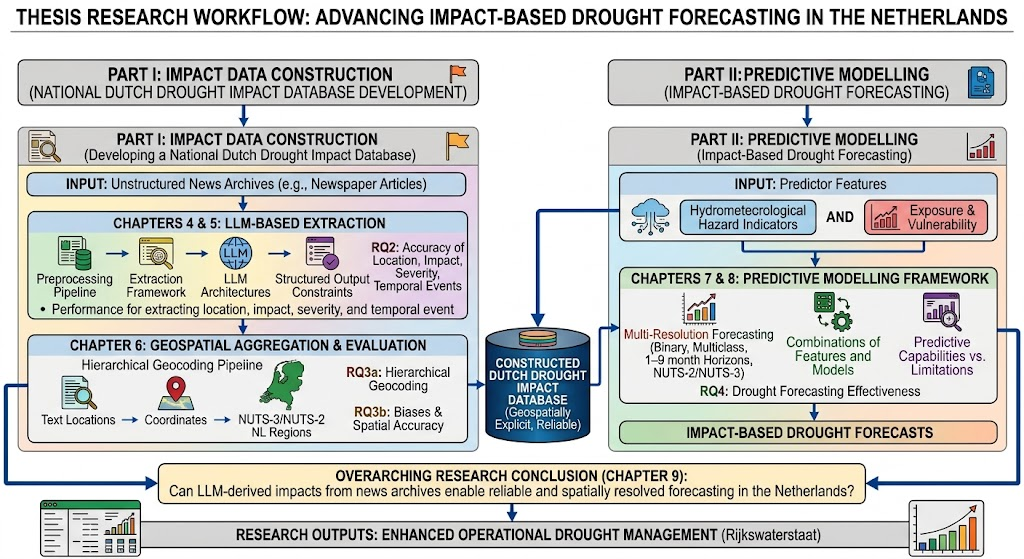
\includegraphics[width=1.05\linewidth]{figures/thesis researcworkflow.jpg}
    \caption{Overview of the research workflow, illustrating the connection between drought impact data construction, evaluation, and impact-based forecasting. [[ik moet de afbeelding nog updaten, staan wat fouten in zoals oude RQ]]}
    \label{fig:researchworkflow}
\end{figure}


The first research component investigates \textbf{(1)} \textit{What are the requirements of impacts of an drought impact dataset satisfy to support regional impact-based forecasting?} This chapter defines the problem and establishes the theoretical data requirements that guide the design of the drought impact database in Chapter~3.



Chapters~4 and~5 focus on the LLM-based extraction of drought impact events. Chapter~4 presents the overall methodology, including the preprocessing pipeline and extraction framework, while Chapter~5 evaluates the performance of different LLM architectures and structured extraction strategies. This component addresses the following research question: \textbf{(2)} \textit{How do different LLM architectures influence the performance of extracting location, impact, severity,
and temporal event information from unstructured text?} The key objective here is to get an reliability measure of our data, since LLMs tend to hallucinate.

Chapter~6 investigates the geospatial aggregation framework that transforms extracted textual information into spatially structured data suitable for predictive modelling. This framework consists of several components, including a point-based geocoding system that converts textual location references into geographic coordinates and an aggregation framework that maps these locations to administrative regions. This enables the extracted information to be represented as spatial features for machine learning applications. The corresponding research question is: \textbf{(3a)} \textit{How can a hierarchical geocoding pipeline be constructed to translate informal textual location references into NUTS-3 and NUTS-2 representations?} In the Netherlands, NUTS-2 regions correspond to the twelve provinces, while NUTS-3 regions represent smaller subregional administrative units. The objective of this aggregation framework is to generate spatial representations that allow machine learning models to identify regional patterns in drought impacts. Subsequently, the resulting database is evaluated to assess its spatial accuracy and reliability through the following research question: \textbf{(3b)} \textit{Which systematic biases, including regional reporting differences and environmental factors, affect the correspondence between news-derived impact data and reference datasets?}


Finally, Chapters~7 and~8 investigate the predictive modelling component of this thesis. This part addresses the following research question: \textbf{(4)} \textit{How effectively can the constructed drought impact database support impact-based drought forecasting in the Netherlands?} [@erik Will probably be changed to a baseline]

These chapters examine which combinations of predictor variables and modelling approaches provide the strongest predictive performance for drought impact forecasting. Model performance is evaluated across multiple spatial, temporal, and classification resolutions, including forecasting horizons ranging from one to nine months, predictions at both the NUTS-2 and NUTS-3 levels, and both binary and multi-class impact prediction tasks. The final chapter synthesises the findings from the preceding chapters and evaluates the broader implications of the proposed forecasting framework. In particular, it examines what the extracted information reveals about drought impacts in practice and discusses its potential contribution to operational drought management in the Netherlands.
